\documentclass[11pt,a4paper,useAMS,iop]{emulateapj}

\usepackage{tikz}
\usetikzlibrary{arrows,shapes,backgrounds}

\usepackage{xcolor}
\usepackage{threeparttable}
\usepackage{multirow}
\usepackage[colorlinks=true,linkcolor=blue,anchorcolor=blue,citecolor=blue,urlcolor=blue,draft=false]{hyperref}
%\usepackage{hyperref}
\bibliographystyle{apj}
\usepackage{amsmath}
\usepackage{graphicx}
\usepackage{morefloats}
\usepackage{natbib}
\usepackage[percent]{overpic}
\usepackage{enumerate}

\newcommand{\vdag}{(v)^\dagger}
\newcommand{\myemail}{gogrean@stanford.edu}

\slugcomment{Submitted to ApJL. Draft version dated \today.}

\shorttitle{The Large-Scale Filament Crossing MACS J0717.5+3745}
\shortauthors{Ogrean et al.}

\newcommand{\chandra}{\emph{Chandra}}
\newcommand{\rosat}{\emph{ROSAT}}
\newcommand{\vla}{\emph{VLA}}
\newcommand{\xmm}{\emph{XMM-Newton}}
\newcommand{\suzaku}{\emph{Suzaku}}
\newcommand{\gmrt}{\emph{GMRT}}
\newcommand{\wsrt}{\emph{WSRT}}

\begin{document}

\title{Frontier Fields Clusters: Origin of the X-ray-Bright Gas \\in the Large-Scale Filament Crossing MACS J0717.5+3745}

\author{
G.~A.~Ogrean\altaffilmark{1, $\dagger$}, C.~Jones\altaffilmark{2}, N.~Werner\altaffilmark{1}, T.~Whalen\altaffilmark{3}, R.~J.~van Weeren\altaffilmark{2, $\ddagger$}, W.~Forman\altaffilmark{2}
}

\affil{\altaffilmark{}}
\affil{\altaffilmark{1}KIPAC, Stanford University, 452 Lomita Mall, Stanford, CA 94305, USA; \href{mailto:gogrean@stanford.edu}{gogrean@stanford.edu}}
\affil{\altaffilmark{2}Harvard-Smithsonian Center for Astrophysics, 60 Garden Street, Cambridge, MA 02138, USA;}
\affil{\altaffilmark{3}University of Maryland, College Park, MD 20742, USA;}

\altaffiltext{$\dagger$}{Hubble Fellow}
\altaffiltext{$\ddagger$}{Clay Fellow}
\altaffiltext{}{}

\begin{abstract}
	We present results from deep \chandra\ observations of the large-scale filament extending SE from the massive Frontier Fields cluster MACS~J0717.5+3745. The filament was previously found to have a length of $\sim 19$ Mpc. Within the filament, about 2~Mpc away from the cluster center, there is a galaxy group with a mass of $\sim 5\times 10^{13}$~M$_\odot$ and a temperature of $\sim 3$~keV. This group is likely infalling for the first time towards the cluster. The filament is brightest in X-ray in the region between the group and the cluster. Here, the gas is found to have a temperature of $1.58_{-0.25}^{+0.51}$~keV and a density of $\sim 10^{-4}$~cm$^{-3}$. The filament density corresponds to a relatively high over-density of $\sim 100$ relative to the critical density of the Universe, which can be explained by the fact that we are probing only the densest part of the filament. The filament properties are consistent with numerical simulations and with the few other observational results reported to date. 
\end{abstract}

\keywords{Galaxies: clusters: individual: MACS J0717.5+3745 --- Galaxies: clusters: intracluster medium --- X-rays: galaxies: clusters}

\section{Introduction}

In the $\Lambda$CDM cosmological model, structure in the Universe is organized in a filamentary web in which large-scale cosmic filaments connect virialized massive structures such as clusters and groups of galaxies \citep[e.g., ][]{Einasto1994}. Approximately a third of the total bayonic matter is expected from hydrodynamic simulations to be contained in these large-scale filaments \citep[e.g.][]{Dave2001}, in the form of low-density gas with temperatures of $10^5-10^7$~K---the warm--hot intergalactic medium (WHIM). One of the main signatures of cosmic filaments is soft X-ray emission. However, the low density of the gas within the filaments poses a significant observational challenge, which causes detections to strongly depend on fortuitous alignments of the filaments with our line of sight. As a consequence, there have been only a handful of filament detections, such as the one in MACS~J0717.5+3745 \citep{Ebeling2004}, the one between A222-A223 \citep{Dietrich2005, Werner2008, Dietrich2012}, and several in A2744 \citep{Eckert2015}.

Clusters of galaxies grow via the infall of gas and the accretion of less massive structures along cosmic filaments \citep[e.g.,][]{Springel2006}. During infall and subsequent collision with the cluster, less massive structures will be ram-pressure stripped as they pass through the cluster's denser regions. Consequently, depending on their original density, these structures are either fully destroyed, or their compact cores survive and develop tails in their wakes. An example of the latter scenario is seen in the cluster 1E~0657--558 \citep{Elvis1992}, in which the collision of a massive cluster with a cluster about $1/10$ of its mass \citep{Springel2007, Mastropietro2008} resulted in the famous ``bullet'' morphology of the less massive structure \citep{Markevitch2002}.

Here, we present results from \chandra\ observations of the merging galaxy cluster MACS~J0717.5+3745. MACS~J0717.5+3745 \citep[$z=0.546$;][]{Ebeling2001, Ebeling2007} is one of the most complex merging systems discovered to date, being the site of collisions between four substructures \citep{Ma2009, Medezinski2013}. The superposition of the dark matter halos of these substructures also makes MACS~J0717.5+3745 the largest known gravitational lens \citep{Zitrin2009, Medezinski2013,Umetsu2014, Umetsu2016}. By analyzing the distribution of galaxies in the cluster region, \citet{Ebeling2004} discovered a large-scale cosmic filament extending SE of MACS~J0717.5+3745. \citet{Jauzac2012} found the filament to be $\sim 19$~Mpc long. Follow-up \chandra\ observations of the intracluster medium (ICM) in the cluster found hot regions with temperatures of $\sim 20$~keV, remnant cool cores with temperatures of $\sim 5$~keV, and density and temperature jumps at the interface between the cluster and the SE filament \citet{Ma2009}. The authors speculated that the jumps are caused by accretion of gas from the filament onto the cluster. The archival \chandra\ observations also revealed a group of galaxies projected onto the large-scale filament, although this structure is not discussed by \citet{Ma2009}. More recently, we have analyzed the thermodynamic properties of the ICM of MACS~J0717.5+3745 using deeper \chandra\ observations (van Weeren et al., submitted). In this letter, we present the physical properties of the SE filament connected to MACS~J0717.5+3745, and those of the group seen in the filament. The analysis is based on the same datasets that were used by van Weeren et al., submitted.

In Section~\ref{sec:DataAnalysis}, we summarize the processing of the \chandra\ datasets. The properties of the group in the filament are discussed in Section~\ref{sec:Group}, while those of the filament are discussed in Section~\ref{sec:Filament}. Our conclusions are summarized in Section~\ref{sec:Summary}.

Throughout the paper we assume a $\Lambda$CDM cosmology with $H_{\rm 0} = 70$~km\;s$^{-1}$\;Mpc$^{-1}$, $\Omega_{\rm m} = 0.3$, and $\Omega_{\rm \Lambda} = 0.7$. For these parameters, 1~arcmin at the redshift of MACS~J0717.5+3745 ($z=0.546$) corresponds to a linear distance of approximately 383~kpc. 


\section{Data Processing and Background Modeling}
\label{sec:DataAnalysis}

\chandra\ observed MACS~J0717.5+3745 four times between Jan~2001 and Dec~2013, for a total of 243~ks. Of the four ObsIDs, two (1655 and 16235) were taken in FAINT mode, while the other two (4200 and 16305) were taken in VFAINT mode. More details about the observation parameters can be found at the \href{http://cda.harvard.edu/chaser/}{Chandra Data Archive}.

The ObsIDs were reprocessed to apply the newest calibration files as of Feb~2016 (v4.7.2). Time periods affected by soft protons were removed from the data using the \textsc{ciao} script \emph{deflare}. ObsID~1655 had residual soft proton flares and therefore we decided to remove it from the spectral analysis. The total clean exposure time after flare filtering was approximately 209~ks (193~ks for the spectral analysis, ignoring ObsID 1655). Point sources were detected in the energy bands $0.5-2$ and $2-7$~keV using the script \emph{wavdetect}, were visually confirmed, and excluded from the analysis. The instrumental background was subtracted using the epoch-specific stowed background files available in the CalDB. Before subtraction, the instrumental background files were normalized to have the same $10-12$~keV count rate as the corresponding source files. 

The sky background was modeled as the sum of unabsorbed emission from the Local Hot Bubble, absorbed emission from the Galactic Halo, and absorbed emission from unresolved X-ray sources. The hydrogen column density was fixed to $8.4\times 10^{20}$~cm$^{-2}$, corresponding to the sum of the atomic and molecular hydrogen column densities in the direction of MACS~J0717.5+3745\footnote{http://www.swift.ac.uk/analysis/nhtot/index.php} \citep{Kalberla2005, Willingale2013}. All the foreground components were assumed to have solar metallicities equal to those reported by\citet{Feldman1992}. All the spectra discussed in the paper were fitted in the energy band $0.5-7$~keV using \textsc{Xspec}.

A more detailed description of the data processing and the background modeling is provided by van Weeren et al., submitted. Our analysis can also be reproduced by the reader by downloading the datasets from the \href{http://cda.harvard.edu/chaser/}{Chandra Data Archive} and running the \textsc{Jupyter} notebook\footnote{Running this notebook requires the \href{https://github.com/takluyver/bash\_kernel}{bash\_kernel package}.} available on GitHub at \url{https://goo.gl/7x2pXR}. 


\section{Group in the Filament}
\label{sec:Group}

The group of galaxies within the large-scale filament is located a little over 2~Mpc SE of the cluster center, chosen to be at ${\rm RA} = 07:17:30.025$, ${\rm Dec} = +37:45:18.58$. The small size of the group and its large distance from the cluster implies that it is falling for the first time towards MACS~J0717.5+3745, rather than having traversed the cluster from the NW to the SE.

We measured the temperature and the brightness of the cluster by extracting spectra from an elliptical region shown in Figure~\ref{fig:fil}. We assumed a group metallicity of 0.2 solar. The best-fitting parameters are summarized in Table~\ref{tab:spectra}. The normalization is equivalent to a luminosity of $(1.05\pm 0.09) \times 10^{43}$~erg~s$^{-1}$. Based on the luminosity-mass scaling relations for galaxy groups \citep[e.g.,][]{Connor2014}, the group's luminosity corresponds to a mass of $\sim 5\times 10^{13}$~M$_\odot$.



\section{X-ray Emission from the Filament}
\label{sec:Filament}

\begin{figure*}
    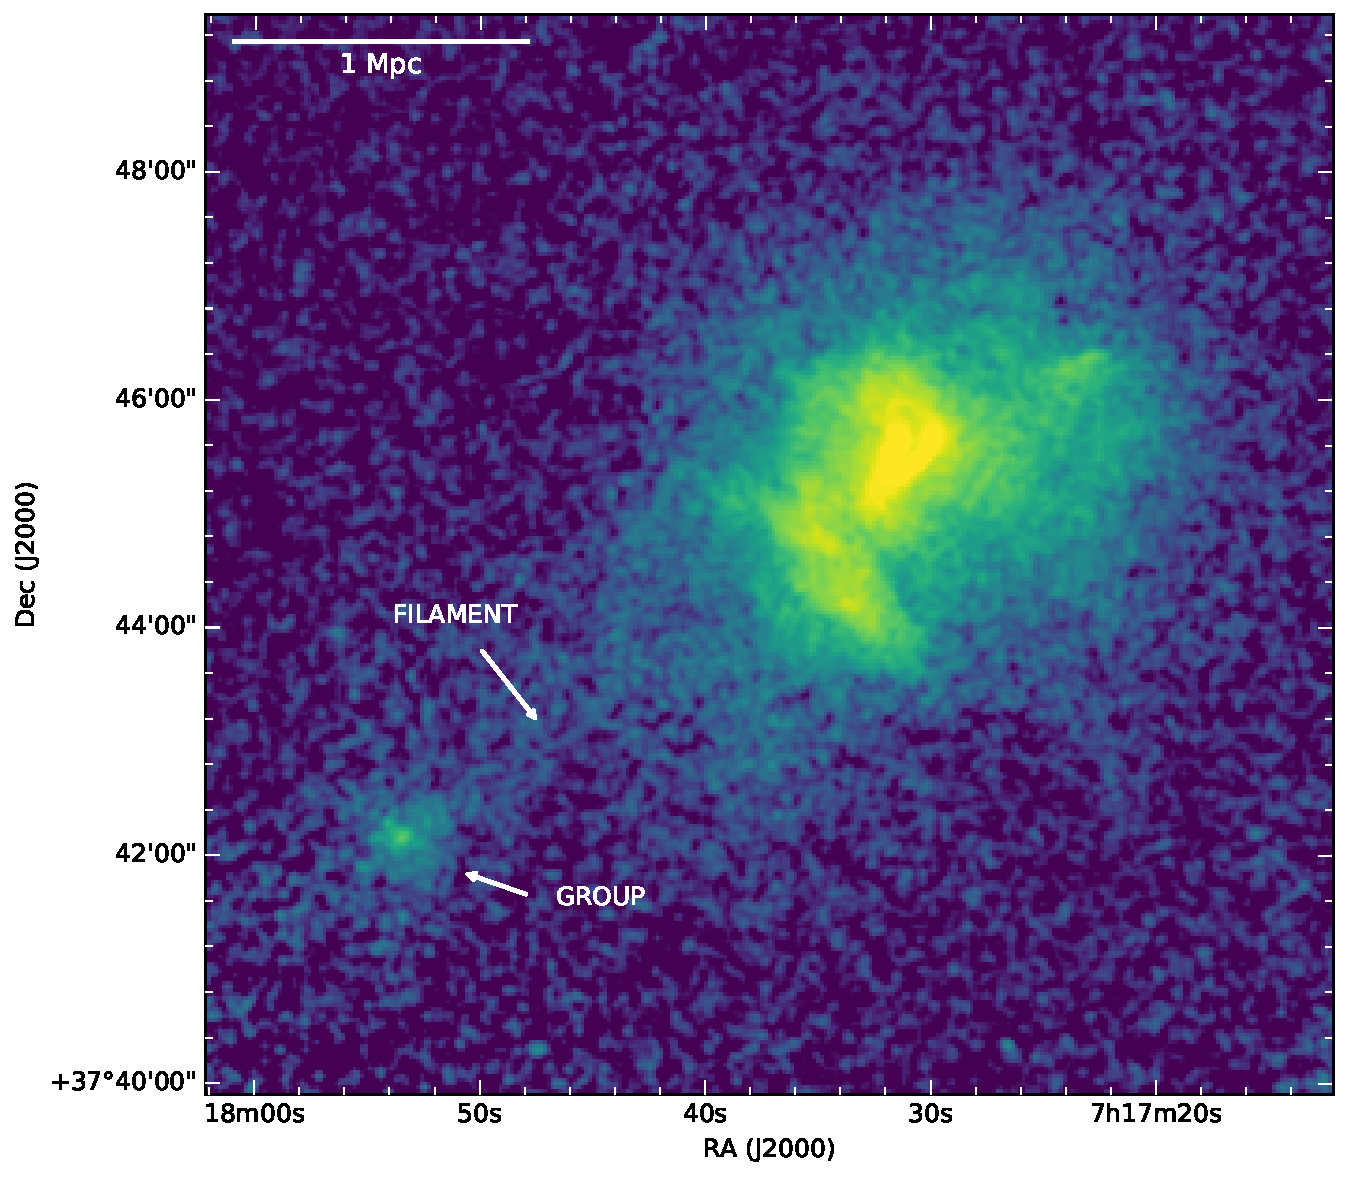
\includegraphics[width=\columnwidth]{plots/fil-labels.pdf}
    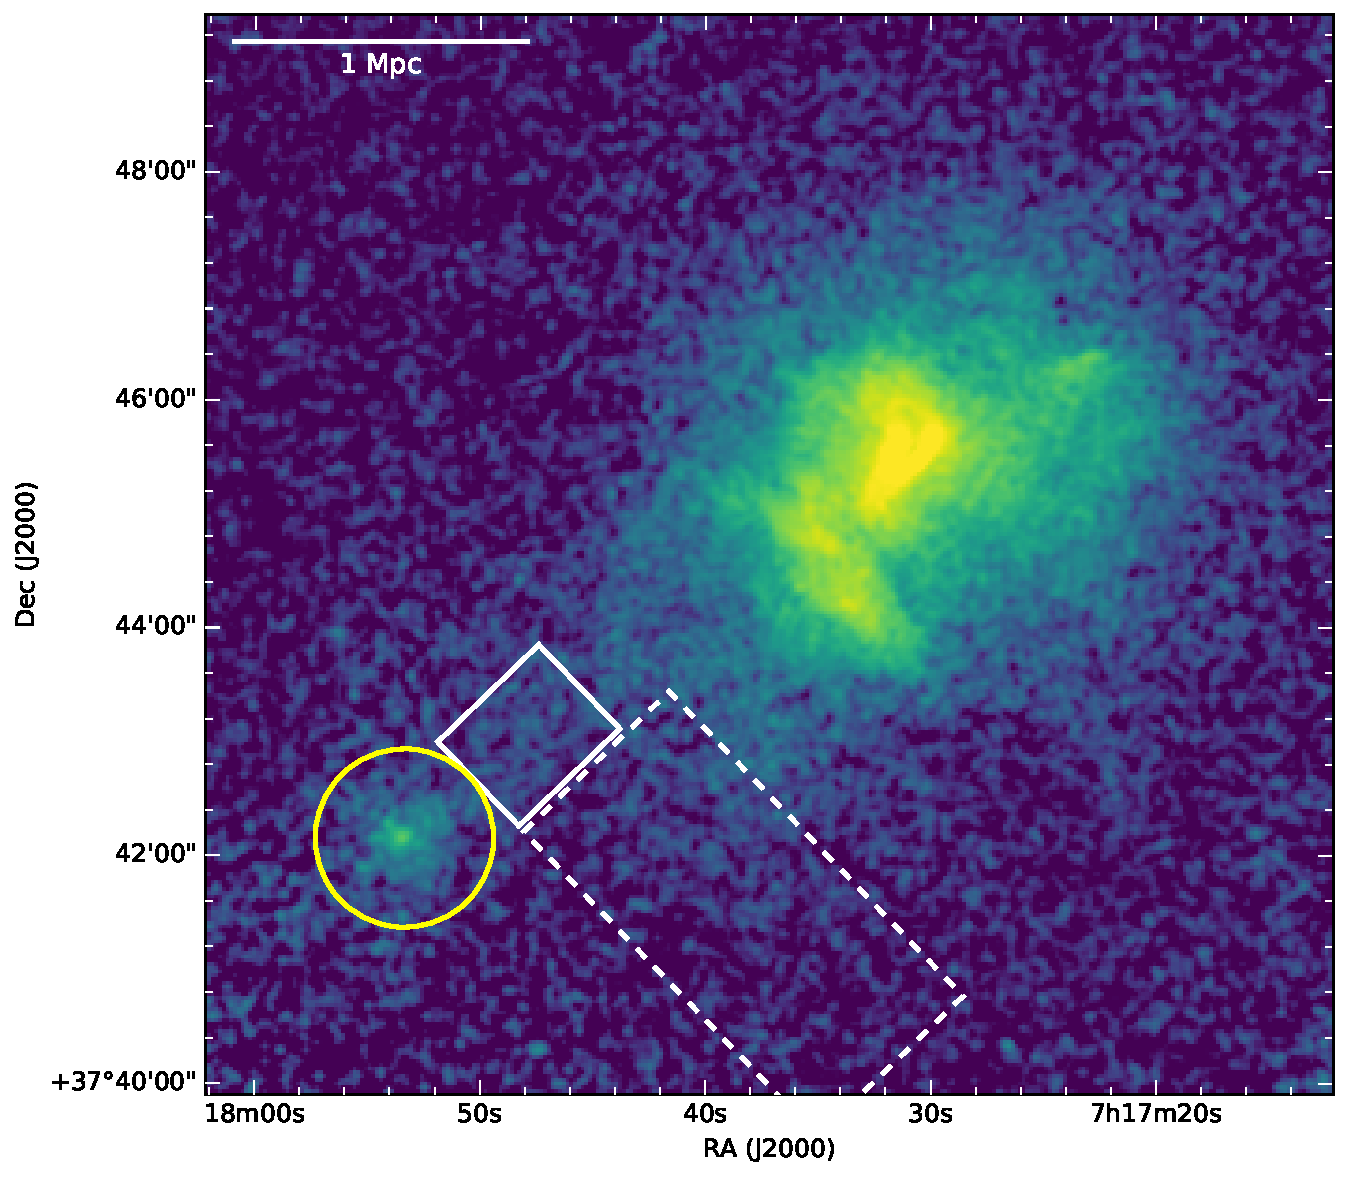
\includegraphics[width=\columnwidth]{plots/fil-regions.pdf}
    \caption{\emph{Left:} Chandra $0.5-4$~keV surface brightness map of MACS J0717.5+3745, showing the features discussed in this work. The image was exposure- and vignetting-corrected. Point sources were subtracted and the gaps were filled by sampling the regions surrounding the point sources. The gaps were filled to create a more visually appealing figure. However, the imaging analysis was done on images that did not have the gaps filled. The images used in the analysis are available online as supporting material. \emph{Right:} Regions used in the spectral analysis. The regions of main interest are drawn in solid lines, while the regions used to characterize the contaminating/surrounding emission are drawn in dashed lines. The best-fitting parameters obtained for the gas in these regions are listed in Table~\ref{tab:spectra}. \label{fig:fil}}
\end{figure*}

\begin{table}
  \caption{Parameters of the regions used for the spectral analysis. The regions are shown in Figure~\ref{fig:fil}. Uncertainties are quoted at the $\Delta C = 1$ level. \label{tab:spectra}}
  \begin{center}
    \begin{threeparttable}
      \begin{tabular}{l c c}
              \multicolumn{3}{c}{\textsc{Foreground and Background}} \\
              \hline\hline
              Model Component & Temperature\tnote{a} & Normalization\tnote{b} \\
              \hline
              Local Hot Bubble & $0.135_{-0.008}^{+0.007}$ & $7.21_{-0.18}^{+0.30} \times 10^{-7}$ \\
              Galactic Halo & $0.59_{-0.08}^{+0.09}$ & $2.78_{-0.44}^{+0.45} \times 10^{-7}$ \\
              Unresolved Background       &\multirow{2}{*}{ -- } & \multirow{2}{*}{ $4.44_{-0.37}^{+0.35} \times 10^{-7}$} \\
              Sources ObsID 16235/16305 &                                    &            \\
              Unresolved Background       &\multirow{2}{*}{ -- } & \multirow{2}{*}{ $7.02_{-0.58}^{+0.49} \times 10^{-7}$} \\
              Sources ObsID 4200               &                                    &            \\
              \multicolumn{3}{c}{} \\
              \multicolumn{3}{c}{\textsc{Large-Scale Filament}} \\
              \hline\hline
                Model Component & Temperature\tnote{a} & Normalization\tnote{b} \\
              \hline
               On Filament & $1.58_{-0.25}^{+0.51}$ & $4.00_{-0.60}^{+0.56} \times 10^{-5}$ \\
               Off Filament & $11.55_{-3.95}^{+9.09}$ & $1.55_{-0.10}^{+0.14} \times 10^{-5}$  \\
               \multicolumn{3}{c}{} \\
              \multicolumn{3}{c}{\textsc{Group in the Filament}} \\
              \hline\hline
                             & Temperature\tnote{a} & Normalization\tnote{b} \\
              \hline
                            & $3.87_{-0.51}^{+0.66}$ & $ ( 1.77\pm 0.13 ) \times 10^{-4}$ \\
              \multicolumn{3}{c}{} \\
              \multicolumn{3}{c}{\textsc{Fly-Through Core}} \\
              \hline\hline
                Model Component & Temperature\tnote{a} & Normalization\tnote{b} \\
              \hline
               Core & $6.82_{-1.36}^{+1.88}$ & $3.41_{-0.25}^{+0.29} \times 10^{-4}$ \\
               N+S of Core & $7.47_{-0.86}^{+1.11}$ & $2.08_{-0.78}^{+0.77} \times 10^{-4}$  \\
               Ahead of Core & $5.06_{-0.98}^{+1.61}$ & $8.52_{-0.77}^{+0.88} \times 10^{-5}$  \\
               Behind Core & $10.89_{-1.27}^{+2.05}$ & $3.92_{-0.09}^{+0.10} \times 10^{-4}$  \\
      \end{tabular}
      \begin{tablenotes}
              \item[a] Units of keV.
              \item[b] Units of cm$^{-5}$~arcmin$^{-2}$ for the thermal components, and photons~keV$^{-1}$~cm$^{-2}$~s$^{-1}$~arcmin$^{-2}$ at 1~keV for the power-law components.
      \end{tablenotes}
    \end{threeparttable}
  \end{center}
\end{table}

To define the region of the filament that is least contaminated by ICM emission, we examined the surface brightness profile in a rectangular region aligned with the filament. In this region, the surface brightness decreases away from the cluster center, and then increases again when the region intersects the SE group located along the filament; there is no radial range in this region where the surface brightness is flat. This suggests that the ICM of MACS~J0717.5+3745 contaminates the filament, and this contamination needs to be considered when modeling the filament emission.

To model the filament and the contamination from the ICM, we extracted spectra in two rectangular regions: one centered on the filament, and one positioned to the SW of it; NE of the filament, the signal-to-noise is too low for any meaningful information to be extracted from the spectrum. These regions are shown in Figure~\ref{fig:fil}. The regions were chosen to avoid the bright parts of the ICM, as well as emission from the SE galaxy group. The emission in the SW region was modeled with a single thermal component, while the emission in the filament region was modeled with two thermal components--one describing ICM contamination, whose parameters were linked to those of the thermal component used to describe the SW region, and one describing emission from the filament. The spectra from the two regions were fitted simultaneously. Table~\ref{tab:spectra} lists the best-fitting parameters obtained for a gas metallicity of 0.2 solar. Varying the metallicity causes only minor changes to the best-fitting parameters, well within the statistical uncertainty ranges. In one of the \textsc{Jupyter} notebooks supporting this letter, we also list the results obtained for metallicities of 0 and 0.1 solar.

The \textsc{XSpec} normalizations of the thermal components listed in Table~\ref{tab:spectra} are defined as:
\begin{equation}
	\mathcal{N} = \frac{n_{\rm e} \, n_{\rm H} \, V}{10^{14} \, \pi \, S_{\rm reg} \, D_{\rm A}^2 \, (1+z)^2} \, , 
\label{eq:norm}
\end{equation}
if we assume the density to be constant in each region, where $n_{\rm e}$ is the electron number density, $n_{\rm H}$ is the hydrogen number density, $V$ is the volume of the region, $S_{\rm reg}$ is the projected area of the region, $D_{\rm A}$ is the angular size distance to the cluster, and $z$ is the cluster redshift.

To calculate the density of the filament in the region shown in Figure~\ref{fig:fil}, we assumed that in 3D the region is a parallelepiped with four rectangular faces: two perpendicular to the line of sight, and two parallel to it. \citet{Jauzac2012}, citing Ebeling et al., in prep., quoted a filament inclination angle $\theta \sim 75$ degrees with respect to the plane of the sky (the results below are highly sensitive to the uncertainty on the inclination angle). They also determined the filament has a diameter $D_{\rm fil} \sim 3$~Mpc at the radius from which our spectra were extracted and a length of $\sim 19$~Mpc. Therefore, the volume of the parallelepiped corresponding to our region is:
\begin{eqnarray}
    V \equiv V_{\rm ppp} = S_{\rm reg} D_{\rm fil} / \cos\theta\, , 
\label{eq:v_ppp}
\end{eqnarray}

The projected region has a length of $1.2$~arcmin ($\approx 460$~kpc) and a width of $1$~arcmin ($\sim 380$~kpc), therefore $S_{\rm reg} = 1.2$~arcmin$^{2}$. Assuming $n_{\rm e} = 1.2\, n_{\rm H}$ \citep[e.g.,][]{Bohringer2010}, and finally substituting Eq.~\ref{eq:v_ppp} in Eq.~\ref{eq:norm}, the electron number density in the X-ray bright part of the filament is $\sim 2\times 10^{-4}$~cm$^{-3}$. The critical density of the Universe at the redshift of MACS~J0717.5+3745 is $1.7\times 10^{-29}$~g~cm$^{-3}$. Assuming the total baryon density is $4.4\%$ the critical density of the Universe \citep{Kirkman2003}, the filament is overdense by a factor of $\sim 450$ compared to the mean baryon density of the Universe. Assuming a baryon mass fraction of $0.15$ \citep[e.g.,][]{Mantz2014}, the mass density of the filament is $\sim 3\times 10^{13}$~M$_{\odot}$~Mpc$^{-3}$. The filament density is therefore in excellent agreement with the density calculated from the weak lensing data by \citet{Jauzac2012} for the same filament geometry. The filament density corresponds to an overdensity of $\sim 100-150$ relative to the critical density of the Universe.\footnote{\citet{Jauzac2012} calculate an overdensity of $206\pm 46$~$\rho_{\rm crit}$, about $65\%$ higher than our value, but this appears to be a miscalculation; our filament mass density values are consistent.}

For the densities calculated above, the mass of the filament in the region from which the spectra were extracted is $\sim 6\times 10^{13}$~M$_\odot$, with $\sim 9\times 10^{12}$~M$_\odot$ in the hot gas. 

\begin{figure*}
    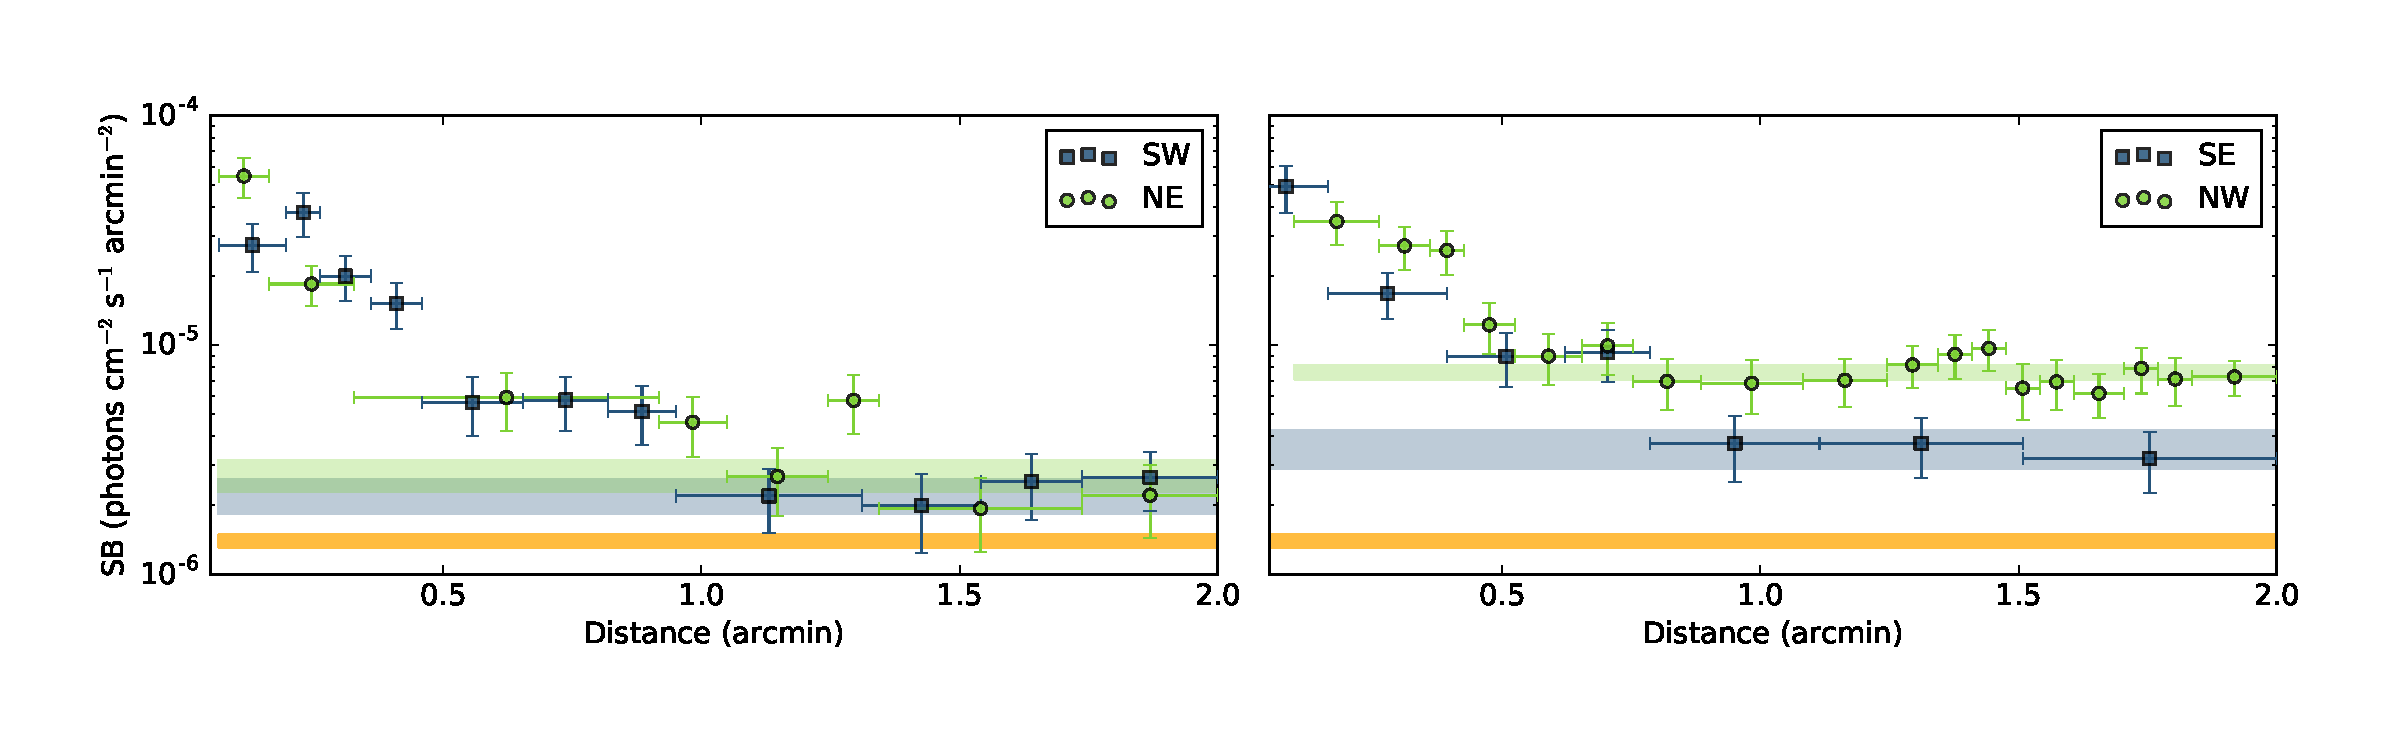
\includegraphics[width=\textwidth]{plots/macsj0717-group-all-directions.pdf}
    \caption{\emph{Top:} Surface brightness profiles perpendicular to (left) and along (right) the filament. The light-colored green and blue bands show the average surface brightness between 1 and 2 arcmin, where the emission from the group is negligible. The orange band shows the $1\sigma$ confidence range of the sky background level. \emph{Bottom:} Sectors from which the surface brightness profiles shown above were extracted. The sectors are centered on the X-ray peak of the galaxy group. \label{fig:group-sx}}
\end{figure*}

In Figure~\ref{fig:group-sx}, we show the surface brightness profiles in four sectors centered on the galaxy group seen within the filament. The surface brightness of the group becomes negligible beyond 1 arcmin. Between 1 and 2 arcmin, the profiles show the NW sector being significantly brighter than the other three; this sector covers the part of the filament between the group and the cluster. On the other side of the group, in the SE sector, the surface brightness between 1 and 2 arcmin is larger than in the SW, but consistent with the surface brightness in the NE sector in the same radial range. The SE sector includes part of the filament at higher cluster-centric radii. The surface brightness here is about twice lower than in the NW sector, which implies a baryon density lower by a factor of $\sim 1.5$ compared to the part of the filament closer to the cluster if the the diameter of the (cylindrical) filament is the same on both sides of the group. However, \citet{Jauzac2012} found that the diameter of the filament might be decreasing by a factor of up to $\sim 2$ from the region ahead of the group to the region beyond the group. If the diameter indeed decreases (the uncertainties on the measurements of \citet{Jauzac2012} are very large), then the decrease could explain the surface brightness difference without a decrease in the filament baryon density.

The calculations made above can be found in one of the supporting \textsc{Jupyter} notebooks accompanying this paper.  







%\section{Fly-Through Core}
\label{sec:FlyThrough}

\begin{figure*}
    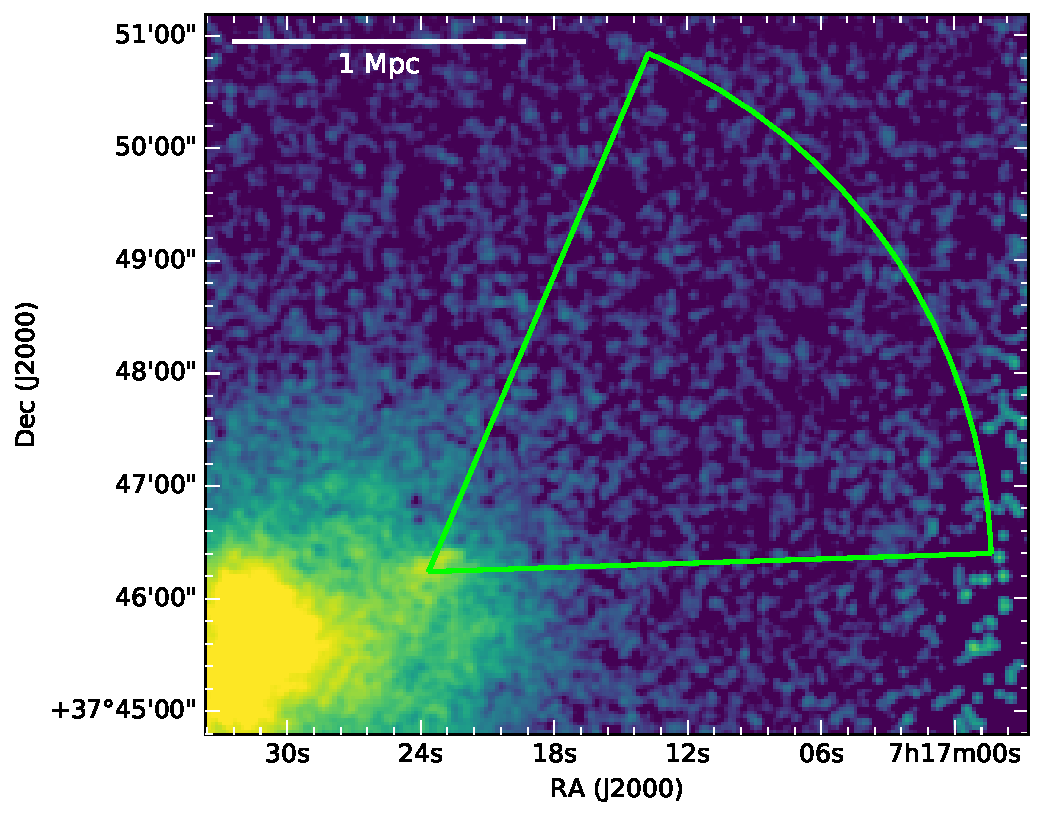
\includegraphics[width=\columnwidth]{plots/circ-panda.pdf}
    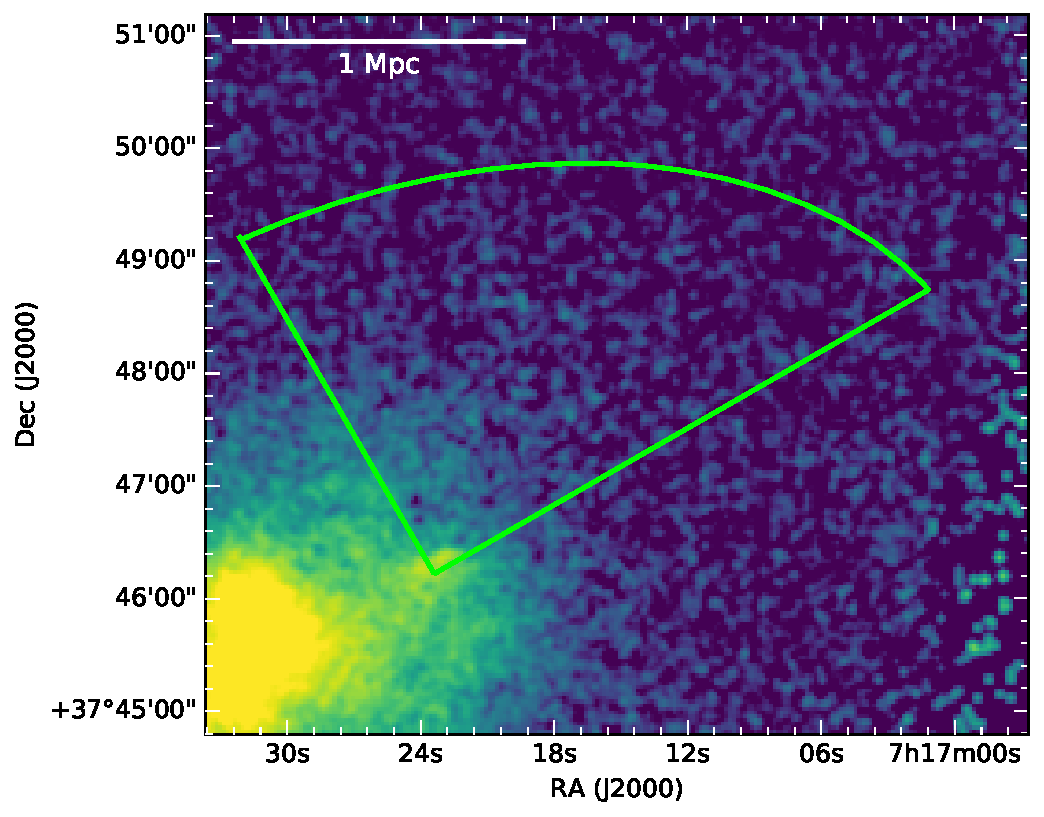
\includegraphics[width=\columnwidth]{plots/ell-panda.pdf}
    \includegraphics[width=0.33\textwidth]{plots/{macsj0717-core-circ-beta}.pdf}
    \includegraphics[width=0.33\textwidth]{plots/{macsj0717-core-ell-beta}.pdf}
    \includegraphics[width=0.33\textwidth]{plots/{macsj0717-core-ell-bknpow}.pdf}
    \caption{\emph{Top:} Sectors used to model the surface brightness profile in front of the core. \emph{Bottom:} Surface brightness profiles and best-fitting models. The instrumental background is shown in blue, with the uncertainty ranges on the background shown in dashed blue lines. For the elliptical sector, the surface brightness is plotted against the major axis of the ellipse. The best-fitting parameters of the broken power-law model are listed in Table~\ref{tab:bknpow}. \label{fig:sectors}}
\end{figure*}

\begin{table*}
  \caption{Best-fitting parameters of the broken power-law model fitted to the surface brightness of the core. Uncertainties are quoted at the $1\sigma$ level. The region from which the surface brightness profile was extracted, as well as the profile and best-fitting model, are shown in Figure~\ref{fig:sectors}.\label{tab:bknpow}}
  \begin{center}
    \begin{threeparttable}
      \begin{tabular}{c c c c c c}
              $\alpha_1$\tnote{a} & $\alpha_2$\tnote{b} & Normalization & $r_{\rm break}$ & $n_1/n_2$\tnote{c} &  Sky background \\
                               &        &     photons cm$^{-2}$ s$^{-1}$ arcmin$^{-2}$       & arcmin   & &    photons cm$^{-2}$ s$^{-1}$ arcmin$^{-2}$ \\
              \hline
              $-0.36 \pm 0.51$ & $1.16 \pm 0.08$ & $(4.97 \pm 1.51)  \times 10^{-4}$ & $0.265\pm 0.005$ & $1.88\pm 0.35$ & $(1.30 \pm 0.14) \times 10^{-6} $ \\
      \end{tabular}
      \begin{tablenotes}
              \item[a] Power-law index at $r < r_{\rm break}$.
              \item[b] Power-law index at $r > r_{\rm break}$.
              \item[c] Density jump across the discontinuity.
      \end{tablenotes}
    \end{threeparttable}
  \end{center}
\end{table*}

Approximately 670 kpc NW of the cluster center, there is a bright X-ray core with a tail extending $\sim 200$~kpc towards SE, roughly in the direction of the large-scale filament discussed in Section~\ref{sec:Filament}. This morphology suggests that this core, seen `flying' through the ICM of MACS~J0717.5+3745 and ram-pressured stripped by the cluster's dense ICM, traveled NW along the SE filament and is seen after it traversed the brightest ICM regions. In essence, the core is a later stage of the group currently seen within the filament. 

The core is embedded (at least in projection) in the ICM of MACS~J0717.5+3745. To determine the core's physical properties, we  modeled the contamination from the ICM by extracting spectra N and S of the core. These spectra were modeled with a thermal component with a metallicity of 0.2 solar. We assumed the spectral properties were the same in the N and S regions. The spectra of the core were modeled as the sum of emission from the contaminating ICM and from the core itself. The spectra of the core and of the regions N and S of it were modeled in parallel. The best-fitting results are summarized in Table~\ref{tab:spectra}. The temperature of the core, $6.82_{-1.36}^{+1.88}$~keV, is consistent with the temperatures N and S of the core, in regions that are approximately at the same distance from the cluster center as the core. We also compared the core temperature with the temperatures ahead of (NW) and behind (SE) the core. The temperature decreases from $10.89_{-1.27}^{+2.05}$~keV behind the core, to $5.06_{-0.98}^{+1.61}$~keV ahead of the core. From these temperature measurements, we therefore find no evidence of a core colder than its surroundings, nor of a temperature discontinuity (either a shock or a cold front) ahead of the core. 

A cold front and a shock front would be expected ahead of the core, similarly to the features seen in the Bullet Cluster \citep{Markevitch2002} and in front of the group NGC 4839 infalling into the Coma Cluster \citep{Neumann2001} ***other citation needed here for the cold front***. We searched for possible evidence of a cold/shock front by modeling the surface brightness profile of the group. The sectors from which the surface brightness profiles were extracted are shown in the top panels of Figure~\ref{fig:sectors}. We chose two sectors: a circular sector with an opening aligned with the apparent direction of motion of the core, and an elliptical sector with an opening and ellipticity aligned with a possible edge observed by eye in the surface brightness map. The models fitted to these surface brightness profiles are shown in the bottom panels of Figure~\ref{fig:sectors}. The surface brightness profile extracted from the circular sector is well-fitted by a $\beta$-model. In this profile, there is a suggestion of an edge near $\sim 0.3$~arcmin, but a surface brightness model based on a broken power-law density model did not significantly improve the fit. In the surface brightness profile extracted from the elliptical sector, this possible edge becomes clearer. A $\beta$-model fit to this profile provides a good fit at high radii, but not at distances below $\lesssim 0.5$~arcmin. As seen in the bottom-right panel of Figure~\ref{fig:sectors}, a broken power-law density model follows the data closer. The best-fitting broken power-law density model fitted to the surface brightness profile in the elliptical sector has a density jump of $1.88\pm 0.35$ at $\approx 0.27$~arcmin from the center of the sector. The best-fitting parameters for the broken power-law model are summarized in Table~\ref{tab:bknpow}.

The density discontinuity is at the very edge of the core. Therefore, we speculate that the discontinuity is associated with a cold front rather than with a shock front. The failure to find a temperature discontinuity associated with the density jump is likely due to a combination of poor count statistics and hot gas projected onto the core. The latter would also dampen the observed density jump, in which case our measurement of the jump amplitude is only a lower limit.  




\section{Summary}
\label{sec:Summary}

MACS~J0717.5+3745 ($z=0.546$) is a massive galaxy cluster selected as one of the six Frontier Fields targets. The cluster is the most morphologically complex merger, being the site of collisions between at least four subclusters. SE of the cluster, there is a large-scale cosmic filament that was first reported by \citet{Ebeling2004}. Some of the subclusters involved in the merger have likely traveled along this filament before colliding with the previously existing structure. \citet{Jauzac2012} determined from optical data that the filament is $\sim 19$~Mpc long and $\sim 1.6$~Mpc wide. Part of the filament that is near the cluster is also visible at X-ray wavelengths. So far, the thermodynamic properties of large-scale filaments have only been studied in a handful of merging clusters \citep{Werner2008, Eckert2015, Bulbul2016}. Here, we used deep \chandra\ observations of MACS~J0717.5+3745 to study the properties of the large-scale filament extending SE of the cluster center, and those of the substructures along the filament. Below is a summary of our results:

\begin{itemize}
	\item The filament has a temperature of $1.58_{-0.25}^{+0.51}$~keV and a density of $\sim 10^{-4}$ cm$^{-3}$. These are consistent at the $90\%$ confidence level with the properties of the other filaments studied in X-ray \citep{Werner2008, Eckert2015, Bulbul2016}.
	\item The filament is over-dense by a factor of $\sim 250$ compared to the mean baryon density of the Universe.
	\item The total mass of the filament, assuming a constant density along its full length, is extremely large, $\sim 7\times 10^{14}$~M$_\odot$. For comparison, \citet{Eckert2015} estimated filament masses $<10^{14}$~M$_\odot$. However, our mass estimate,  which relies on the measured gas density, should be considered only an upper limit since the gas density is expected to decrease with increasing distance from the cluster.
	\item A little over $2$~Mpc SE of the cluster center, embedded within the filament, there is a galaxy group with a temperature of $\sim 3$~keV and an X-ray luminosity of $\sim 10^{43}$~erg~s$^{-1}$ in the energy band $0.1-2.4$~keV. The mass of the group is estimated to be $\sim 5\times 10^{13}$~M$_\odot$. This group is very likely to be approaching the cluster for the first time.
	\item Approximately $670$~kpc NW of the cluster center, there is a ram pressure-stripped core with a temperature of $\sim 7$~keV. This core is a remnant of a substructure that already collided with the cluster and traversed the densest regions of the ICM. On the N-NE edge of the core, we detect a density discontinuity that is likely associated with a cold front. However, projection effects and poor count statistics in this region prevent us from detecting a temperature jump that would be needed to confirm the nature of the density discontinuity.
\end{itemize}

\acknowledgments
GAO acknowledges support by NASA through a Hubble Fellowship grant HST-HF2-51345.001-A awarded by the Space Telescope Science Institute, which is operated by the Association of Universities for Research in Astronomy, Incorporated, under NASA contract NAS5-26555. RJvW is supported by a Clay Fellowship awarded by the Harvard-Smithsonian Center for Astrophysics. FAS acknowledges support from \chandra\ grant GO3-14131X.

This research made use of \textsc{APLpy}, an open-source plotting package for \textsc{Python} hosted at \url{http://aplpy.github.com}, and of \textsc{Astropy}, a community-developed core \textsc{Python} package
  for Astronomy \citep{astropy}. This research has also made use of NASA's Astrophysics Data System, and of the cosmology calculator developed by N. Wright \citep{Wright2006}. The \chandra\ data was obtained from the Chandra Data Archive, and analyzed using software provided by the Chandra X-ray Center (CXC) in the application packages \textsc{CIAO} and \textsc{ChIPS}. The X-ray surface brightness profiles were created with \textsc{PyXel} (available at \url{https://github.com/gogrean/pyxel}) and plotted using \textsc{matplotlib}, a \textsc{Python} library for publication quality graphics \citep{Hunter2007}.
  
 The optical data shown in the paper is based on observations made with the NASA/ESA Hubble Space Telescope, and obtained from the \href{http://hla.stsci.edu/}{Hubble Legacy Archive}, which is a collaboration between the Space Telescope Science Institute (STScI/NASA), the Space Telescope European Coordinating Facility (ST-ECF/ESA) and the Canadian Astronomy Data Centre (CADC/NRC/CSA).


\bibliography{fil}
\clearpage

\end{document}




